\chapter{Desarrollo}

\section{Utilizando Excel, para los datos de la pregunta 5, encuentre una regresión lineal y una cuadrática a los datos y los respectivos coeficiente de determinación (R2). ¿Cuál es mejor?}

Para el análisis de datos con el fotocolorimetro Neulog se consideraron las muestras de color azul y la configuración en el dispositivo con el led rojo, obteniendo de esta forma para cada concentración las absorbancias mostrada en la figura \ref{fig:abs-lineal}.

\begin{figure}
	\centering
	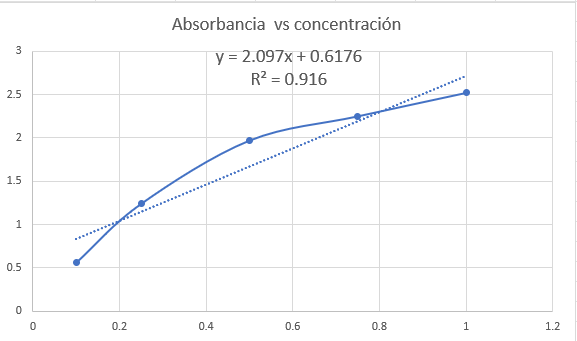
\includegraphics[width=0.7\linewidth]{media/abs-lineal}
	\caption{Regresión lineal - Absorbancia vs concentración}
	\label{fig:abs-lineal}
\end{figure}

\begin{figure}
	\centering
	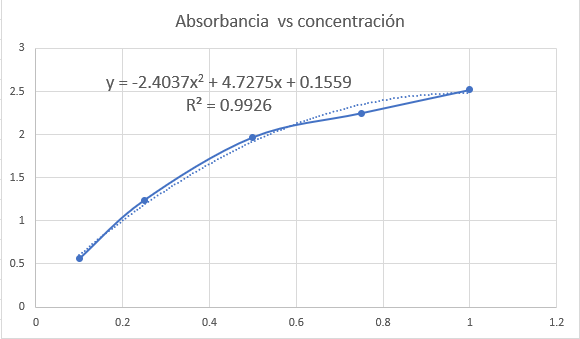
\includegraphics[width=0.7\linewidth]{media/abs-polinomica}
	\caption{Regresión polinómica - Absorbancia vs concentración}
	\label{fig:abs-polinomica}
\end{figure}

Como se describen en las figuras \ref{fig:abs-lineal} y \ref{fig:abs-polinomica} el comportamiento de la absorbancia respecto a la concentración es no lineal con una aproximación a una curva polinomica de 2do orden esto en función al coeficiente de determinación el cual describe de mejor manera los datos en un 99.26\%, siendo este el mejor modelo en comparación al lineal que cuenta con un coeficiente del 91.6\%.

\begin{figure}[h]
	\centering
	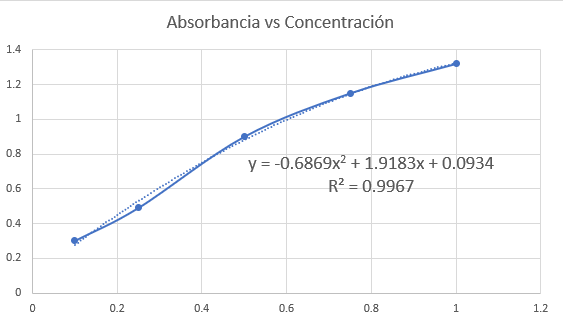
\includegraphics[width=0.7\linewidth]{media/abs-pol-verde}
	\caption{}
	\label{fig:abs-pol-verde}
\end{figure}

La conclusión obtenida se comprueba con el análisis de los datos para las muestras de color verde cuyas absorbancias y comportamiento respecto a la concentración también muestran una tendencia polinómica con un coeficiente de determinación del 99.67\% para el polinomio de 2do orden.

\section{Para el problema inverso dada una absorbancia, calcular la concentración respectivas (\%), vuelva a aplicar el ajuste de curvas pero como variable independiente tendrá absorbancia y como variable dependiente la concentración. Escriba las funciones lineal y cuadrática respectiva.}

Para el problema inverso se obtuvo la inversa de cada función la cuya de forma simplificada se obtiene cambiando los ejes obteniendo en cada las gráficas de la concentración vs absorbancia para las muestras azules, verdes según lo analizado previamente y cuyas gráficas se muestras en la figuras \ref{fig:conc-lineal-azul}, \ref{fig:conc-pol-azul}, \ref{fig:conc-lineal-verde}, \ref{fig:conc-pol-verde}.


\begin{figure}
	\centering
	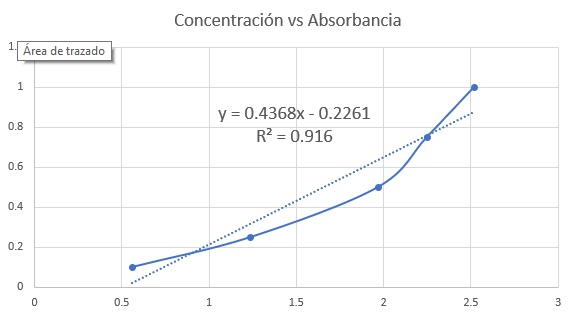
\includegraphics[width=0.7\linewidth]{media/conc-lineal-azul}
	\caption{}
	\label{fig:conc-lineal-azul}
\end{figure}

\begin{figure}
	\centering
	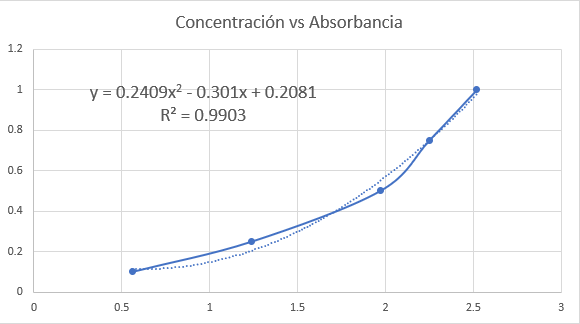
\includegraphics[width=0.7\linewidth]{media/conc-pol-azul}
	\caption{}
	\label{fig:conc-pol-azul}
\end{figure}

\begin{figure}
	\centering
	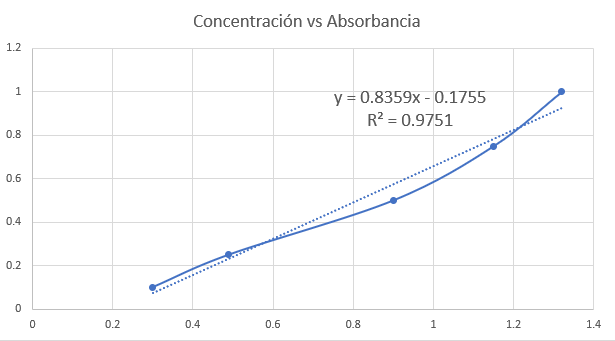
\includegraphics[width=0.7\linewidth]{media/conc-lineal-verde}
	\caption{}
	\label{fig:conc-lineal-verde}
\end{figure}

\begin{figure}
	\centering
	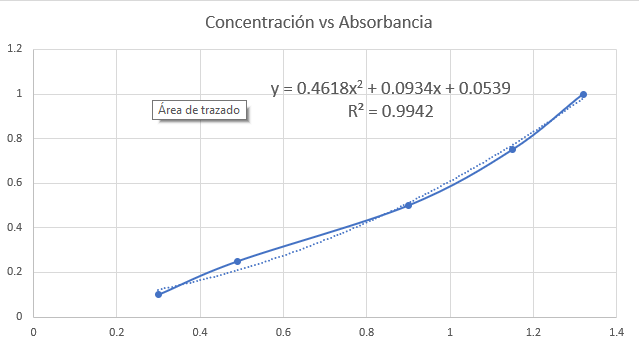
\includegraphics[width=0.7\linewidth]{media/conc-pol-verde}
	\caption{}
	\label{fig:conc-pol-verde}
\end{figure}

























